\chapter{Higgs decaying to two photons}


\section{Object Reconstruction and Identification}

\subsection{Photon Energy Reconstruction}

The natural width of the Higgs for at low mass is negligible when compared to the experimental 
resolution of the calorimeter. 

$\approx$ 6-8 pages in total just using information from PAS + Notes
subsections on photon selection and vertex selection.

MC / data comparison plots

Event selection
After applying the selection, the majority of the remaining background comprises of real 


\section{Signal Extraction}

The signature for the decay $\Hgg$ is the presence of a narrow peak on a smoothly falling background in 
the invariant mass spectrum. 
The signal to background ratio can be dramatically increased by focusing on events falling in a window 
around the mass of the Higgs boson, $m_{H}$. Since this mass is unconstrained in the Standard Model, 
the search is perfomed for a range of mass hypotheses effectively sliding the signal window across 
the diphoton mass spectrum.

As the signal yield for a SM Higgs decaying to two photons is expected to be small, 
additional event information from the detector and the kinematics of the diphoton system can be used to 
increase the sensitivity of the search. 

This section descibes a MVA based approach to extracting the signal, categorizing events within a sliding 
signal region window based on a single event discriminator. The approach allows for use of data in sidebands
to determine expected event yeilds within the signal region, making little assumption about the specific
composition and kinematics of the background. 

\subsection{Definition of the Signal region}

Once the expected resolution of the Higgs peak is determined, the choice of signal window can be optimized
to reduce the uncertainty on the background while selecting as many signal events as possible.
The size of the signal window is chosen using a simplified analysis in which the number of signal events
from a SM Higgs with hypothesised mass $m_{H}$ expected within the range $|\Delta M/M_{H}|=|(\mgg-m_{H})/m_{H}| < w$ 
is compared to the uncertainty on the total number of events (from background and signal) in that range.
The figure of merit, $N_{S}/\sigma = N_{S}/\sqrt{\sigma_{S}^{2} + \sigma_{B}^{2}}$, is calculated as
a function of signal region cut value, $w$, for a range of mass hypotheses as shown in Figure
%~\ref{fig:sigwindowopt}
The error on the background is calculated using the procedure defined in whereas the error on the signal is 
purely statistical.
%\ref{} where the background modelling is done

\begin{figure}
 \begin{centering}
  \includegraphics[width=\textwidth]{hgg7TeV/sidebandMvaPlots/fom.png}
 \end{centering}
  \caption{Figure of merit for selection of the signal region cut value, $w$. Each color shows the evaluation
  under different Higgs mass hypotheses.}
  \label{fig:sigwindowopt}
\end{figure}

For this analysis, $w=0.02$ was chosen as the optimal signal region cut value.

\subsection{Event BDT Desciminator}

The inputs to the diphoton BDT contain information from the event kinematics and the quality of the photons 
and vertex location in the form of the photon ID MVA output and event resolution estimators. 
The output of the diphoton BDT combined with the invariant mass of the diphoton system therefore provides 
the necessary information to separate signal from background.

Figure
%~\ref{fig:bdtplane} 
shows the variation in the signal to background ratio across different regions in the 
two-dimensional plane defined by the output of the diphoton MVA and $\dmom$.

\begin{figure}
 \begin{centering}
  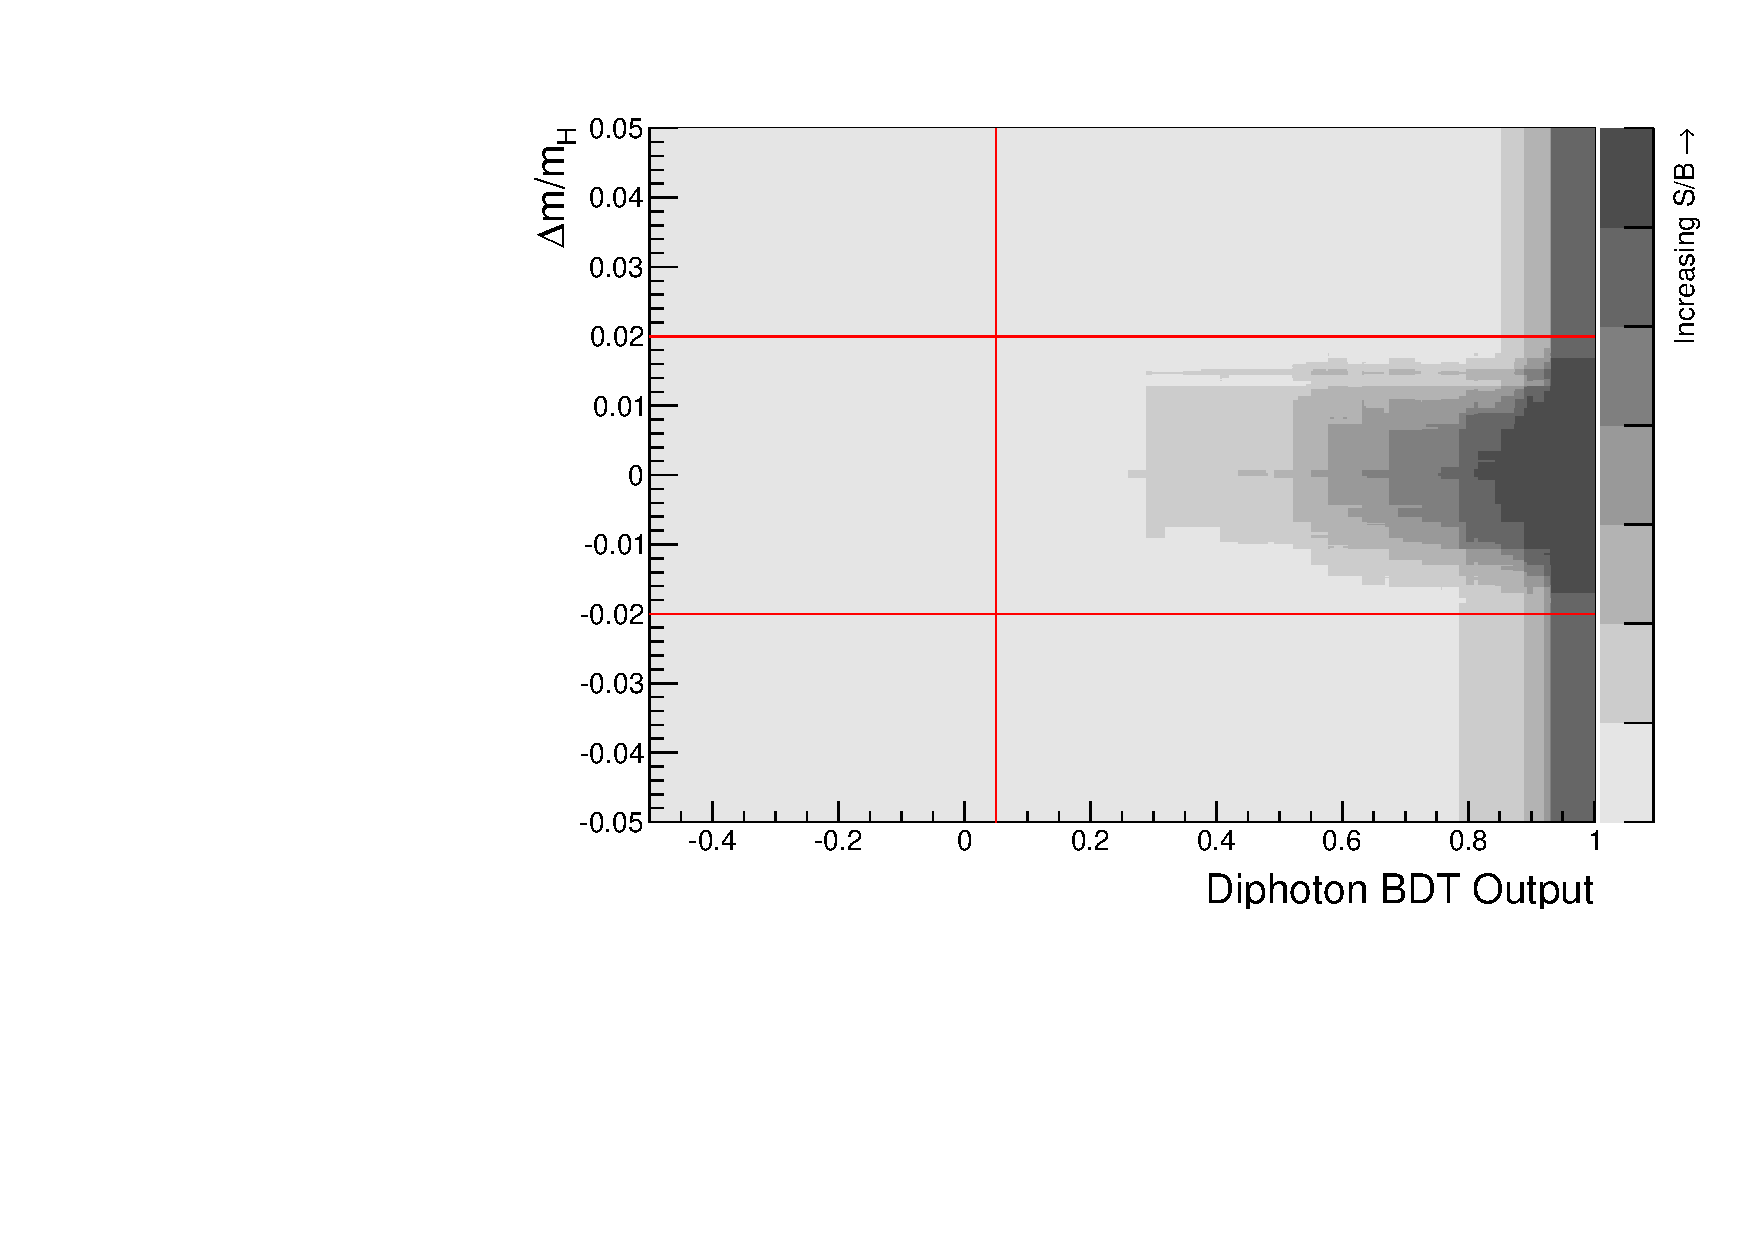
\includegraphics[width=\textwidth]{hgg7TeV/sidebandMvaPlots/bdt2dplot.png}
 \end{centering}
 \caption{Signal to background ratio as a function of diphoton BDT output and $\dmom$.
 The red lines indicate the cuts applied before the training and for applying the event selection.}
 \label{fig:bdtplane}
\end{figure}

The two variables are combined to produce a single event disctiminator by training a BDT with TMVA using the diphoton BDT output and $\dmom$ as inputs.
The BDT is trained with Higgs signal MC with $m_{H}=123$ GeV including all four production processes and background MC including prompt-prompt, prompt-fake
and fake-fake events.

% ? Some description about the two training techniques maybe ? or it might be better in the Introduction to the H->gg section?
The performance of several different training methodologies were compared to find which gave the optimum separation of signal and background.
Two different choices of boosting were studied, one in which BLAH BLAH (adaptive boosting) and the other BLAH BLAH (gradient boosting).
In addition, these were compared to a simple likelihood and decorrelated likelihood (which considers at most linear correlations between the variables)
as shown in Figure
%~\ref{fig:mvacomparisons}.
The gradient boosting method was found to give the best performance although the variation between methodologies was small.
 

%With finite statistics, a BDT can be overtrained by allowing the training to emphasise statistical fluctuations which are not physical and will not necessarily be
%representative of the data. To test for this, the MC samples are split into two equal samples, the first of which is used to train the BDT. The second set are 
%then used to evaluate the BDT's overtraining by comparing their distribution to that of the training sample using a Kolmogorov-Smirnoff (KS) test.
%The distributions for the train and test sample for signal and background shown in Figure~\ref{fig:bdttraining}.
%The KS test is calculated using a very fine binning (5000 bins) to avoid dependance of the test on binning choice.

%\begin{figure}
% \begin{centering}
%  \includegraphics[width=\textwidth]{hgg7TeV/sidebandMvaPlots/bdttraining.png}
% \end{centering}
% \caption{Signal and background BDT output distribution with the training sample (points)
%and testing sample (solid area) superimposed using an arbitary uniform binning.}
% \label{fig:bdttraining}
%\end{figure}

In this analysis, the background is estimated entirely from data. This means that any disagreement between
data and MC will only effect the performance of the BDT and not the validity of the final results. 
The agreement between the data and MC is shown in Figure~\ref{fig:datamcagreement_sidebandBDT} for a mass 
hypothesis, $m_{H}=145$ GeV. The level of agreement is sufficient so as not to require indepth study of the
BDT output distribution of the background MC.

\begin{figure}
 \begin{centering}
  \includegraphics[width=\textwidth]{hgg7TeV/sidebandMvaPlots/data-mc-sbsum-mh145}
 \end{centering}
 \caption{Distribution of data and MC in BDT output for $m_{H}=145$ GeV, binned in constant bin width.}
 \label{fig:datamcagreement_sidebandBDT}
\end{figure}

\subsection{Binning of the BDT Output Distribution}

The BDT provides a single variable with which to classify events based on their signal to back-
ground ratio which will have a discrete number of response values based on the number of
trees used. The boosting procedure provides a pseudo-continuous distribution which is used
to model the signal and background. However, the resulting distribution will still be only
pseudo-continuous. In addition, the BDT response does not directly correspond to a physical
distribution and it is therefore difficult to motivate any parameterisation of either the signal
or background distributions. To overcome these issues, a binning procedure is defined to con-
struct templates which are used as models for the signal and background expectation as a
function of BDT response range (BDT bin). This procedure is designed firstly to ensure that no
bin in the data-driven background model is empty and secondly that as few bins as possible
are used without reducing too much the sensitivity of the BDT to improve performance of the
limit calculation and allow for better modelling of systematic variations.

The binning procedure is defined as follows:

\begin{enumerate}

\item The distribution of background MC is binned very finely to provide an almost discrete
dataset (5000 equally spaced bins are used). The background is re-binned such that there are 20
expected events per bin at a luminosity of \clumi. The procedure starts from the highest BDT
value bin since the final step bin may have less than 20 events. If that is the case, the last and
penultimate bins are combined.
\item Smoothed versions of the signal (at each 5 GeV step mass) and background MC tem-
plates are produced in order to obtain a stable model of the signal to background ratio
$S/B$ as a function of BDT bin.
The smoothing procedure is done via binning a fit (of a 9th order polynomial) to the signal
distribution. Other smoothing techniques were found to give less stable performance.
\item $N$ bin edges (boundaries), $b_{i}$, are defined on the remaining bins such that $N+1$ bin-
ranges (categories) are formed with $b_{1} < b_{2} < \ldots < b_{N}$. A full scan is performed varying the
bin edges to find the maximum expected significance in the presence of a SM Higgs signal. 
\item An extra boundary is added and the scan is repeated and the maximum expected
significance is found for $N+1$ boundaries. If the maximum expected significance  
is increased by more than 0.1\% compared to that of step 3, the new boundary is kept and step 4 
is repeated, if not, the procedure terminates.
\end{enumerate}

The scan in step 3 is split into two parts, first using a large step size to find the 
region where the maximum lies
and then small steps within that region. The ratio of small to large step size is chosen to be that
which minimizes the total number of iterations in the scan reducing the time taken for the procedure.
An example of the binning procedure is shown in Figure~\ref{fig:binningscheme}. 
The red histogram is the $S/B$ distribution after step 1, the 
blue after step 2 and the black vertical lines show the final set of 7 bins chosen for this analysis.

\begin{figure}
 \begin{centering}
  \includegraphics[width=0.9\textwidth]{hgg7TeV/sidebandMvaPlots/binningscheme.png}
 \end{centering}
 \caption{Signal to background ratio as a function of BDT output bin.
 The red and blue histograms show the distribution after applying step 1 of the binning procedure before
and after smoothing respectively. The black vertical lines indicate the boundaries of the final
binning choice from the full procedure.}
 \label{fig:binningscheme}
\end{figure}



\subsection{Background modelling}

$\approx$ 4-5 pages. Datafits to sidebands ,
systematic studies on background normalization
and shape (linear, 2nd order pol \ldots)

\subsection{Signal modelling}
$\approx$ 4-5 pages describing systematics and how they are included into 
the model. Describe relevant measurements from Z's.

\subsection{7TeV results}
$\approx$ 1 pages limits, pvalues \ldots
Since the mass of the Higgs is unknown, the data are tested against a range of possible mass hypotheses

\section{8TeV results}
$\approx$ 1-2 pages, describing changes to analysis in 2012,
resutls from 2012 + combined with 2011 
